\documentclass[a4paper,12pt]{article}

% --------------------------------------------------
% Пакеты
% --------------------------------------------------
\usepackage[resetfonts]{cmap}   % корректная копия шрифтов в pdf
\usepackage[utf8]{inputenc}     % кодировка исходника
\usepackage[T2A]{fontenc}       % кодировка шрифтов
\usepackage[russian]{babel}     % переносы и локализация
\usepackage{indentfirst}        % абзацный отступ в первом абзаце
\usepackage{csquotes}           % корректные кавычки
\usepackage[super]{cite}        % ссылки в виде верхних цифр
\usepackage{hyperref}           % кликабельные ссылки
\usepackage{graphicx}           % рисунки
\usepackage{amsmath,amssymb}
\usepackage{multirow}
\usepackage{geometry}
\geometry{margin=2.5cm}

% чёрные ссылки, без рамок
\hypersetup{
    colorlinks=true,
    linkcolor=black,
    citecolor=black,
    urlcolor=black
}

% --------------------------------------------------
\begin{document}

\begin{titlepage}
	
	 \vspace{-0.7 in}
	\begin{center}
		\begin{figure}[h!]
			\centering
			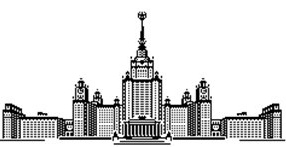
\includegraphics[width = 6cm, height = 4 cm]{msu.jpg}
			\label{fig:msu}
		\end{figure}
		\normalsize{{Московский  государственный
				университет имени М.В.~Ломоносова}}\\[0.1cm]
		\normalsize{{Факультет космических исследований}}\\[0.1 cm]
  \normalsize{{Специальность 01.05.01 <<Фундаментальные математика и механика>>}}\\[0.1 cm]
\normalsize{{ Образовательная программа <<Космические исследования и космонавтика>>}}
		\noindent\rule{16cm}{0.4pt}
		\vfill
	
		\hfill \break
		\textbf{\Large{Нейросетевые методы для декодирования тонкой моторики по биоэлектрической активности}}\\ [0.3cm]
        \normalsize{{Курсовая работа}}\\
		\vfill
		\normalsize
		\begin{flushright}
			Выполнил студент 3 курса группы 302\\
			Балановский Антон Леонидович\\
			
			 
			
			Научный руководитель\\
			\textcolor{red}{НАПОМНИТЕ РЕГАЛИИ,}\\
            Лебедев Михаил Альбертович\\

			
		\end{flushright}
		\hfill \break
	\end{center}
	
	\vfill
	\begin{center}{Москва, 2024}\end{center}
	\thispagestyle{empty} 
	%\setlength{\headsep}{0.2in}
\end{titlepage}
\newpage

% Содержание
\renewcommand{\contentsname}{Содержание}
\tableofcontents

\newpage

% --------------------------------------------------
% ВВЕДЕНИЕ
% --------------------------------------------------
\addcontentsline{toc}{section}{Введение}
\section*{Введение}

Электромиография (ЭМГ) — метод регистрации биопотенциалов, возникающих при сокращении мышечных волокон. Он широко применяется как в фундаментальных физиологических исследованиях, так и в прикладных задачах спорта и реабилитации. Подробная методика наложения электродов, подавления помех и интерпретации сигналов детально описана в работе\,\cite{kostyuchenko2007}, где показано, как получать достоверные ЭМГ‑записи даже во время динамических упражнений.

Точное и устойчивое распознавание ЭМГ‑сигналов открывает целый спектр практических применений. Одно из наиболее заметных — управление протезами конечностей: утерянное движение воспроизводится за счёт «чтения» остаточной мышечной активности. Принцип работы таких систем и результаты экспериментальных прототипов изложены в статьях\,\cite{sudarsan2012,parajuli2019}, где обсуждаются преимущества, ограничения и возможные пути улучшения миоэлектрического управления.

Не менее важна и диагностическая сторона ЭМГ. Поверхностные сигналы позволяют отличать нормальную мышечную активность от патологической и тем самым поддерживать раннюю диагностику нервно‑мышечных заболеваний. Так, Sadikoglu и соавт. показали, что даже простые спектро‑временные признаки позволяют автоматически классифицировать ЭМГ и выявлять нейропатию с точностью выше 90~\%\,\cite{sadikoglu2017}. Исмайлова\,\cite{ismailova2019} дополнительно продемонстрировала, что оптимальный подбор функции ошибки и метода её минимизации заметно повышает чувствительность моделей при диагностике миопатий. Для центральных нарушений, в частности болезни Паркинсона, Meigal и коллеги предложили использовать нелинейные параметры (энтропия, фрактальная размерность) — они меняются уже на доклинической стадии и помогают различать паркинсонический и эссенциальный тремор\,\cite{meigal2013}. Благодаря подобным работам ЭМГ укрепляется как удобный и недорогой инструмент раннего скрининга и мониторинга прогрессирования нервно‑мышечных расстройств.

Несмотря на то, что задачу классификации ЭМГ можно отнести к алгоритмически разрешимым — при фиксированном числе жестов и конечной длине записи всегда существует конечный алгоритм, который выдаст правильную метку за конечное число шагов — на практике она остаётся крайне трудной для традиционных методов. Причина — в высокой изменчивости самих сигналов. На их форму одновременно влияют:
\begin{itemize}
    \item физиологические различия между людьми (толщина подкожного жира, сила мышц, тонус);
    \item точное положение и поворот электродов на коже, которое неминуемо дрейфует даже в течение одной сессии;
    \item внешние помехи (сетевой гул, движение кабелей, потение кожи) и внутренний шум аппаратуры.
\end{itemize}

Данная работа опирается на статью\,\cite{linderman2009}, где была исследована возможность восстановления почерка из данных ЭМГ и продемонстрировано, что поверхностная ЭМГ руки и предплечья содержит достаточно информации для восстановления реальной траектории пера и для прямой классификации символов.

\newpage

% --------------------------------------------------
% ЦЕЛЬ РАБОТЫ
% --------------------------------------------------
\section{Цель работы}
Экспериментально оценить свёрточную нейронную модель на способность классифицировать многоканальные поверхностные ЭМГ‑сигналы.

\newpage

% --------------------------------------------------
% МЕТОДЫ
% --------------------------------------------------
\section{Методы}

\subsection{Экспериментальный дизайн}

\paragraph{Участники и запись данных.} В исследовании участвовали шесть здоровых добровольцев. С восьми биполярных электродов (4 мышцы предплечья + 4 мышцы кисти) регистрировалась ЭМГ с частотой 1~кГц; координаты пера фиксировались планшетом Wacom. Каждый испытуемый записывал цифры «0–9» по 50 повторов.

\paragraph{Алгоритмы.}
\begin{enumerate}
    \item \textbf{Реконструкция траектории}: линейный фильтр Винера, моделирующий координаты $X,\,Y$ пера как взвешенную сумму отстающих и опережающих выборок прямоугольной ЭМГ.
    \item \textbf{Классификация символов}: разбиение записи на эпизоды письма по суммарной ЭМГ $\rightarrow$ выделение 3{,}5‑с окон $\rightarrow$ ПКА $\rightarrow$ линейный дискриминантный анализ (LDA).
\end{enumerate}

Настоящая курсовая наследует датасет из вышеописанной работы, однако вместо LDA используется CNN, что позволяет обрабатывать нелинейные взаимосвязи между каналами. Это должно
\begin{itemize}
    \item повысить среднюю точность;
    \item улучшить переносимость на данные, полученные от других людей (в исходном наборе 6 испытуемых);
    \item заложить основу для дальнейшего перехода на более эффективные трансформеры.
\end{itemize}

\subsection{Формат исходных данных}
Электромиограмма регистрировалась с восьми поверхностных биполярных электродов, расположенных продольно вдоль основных мышечных групп предплечья и кисти. Частота дискретизации выбрана $f_{\!s}=1000$~Гц; сырые отсчёты сохранялись в микровольтах (µV) в матрице размера $(N,8)$, где $N$ — число сэмплов записи, 8 — количество каналов. Также сохранялся рисуемый объект, номер итерации и положение пера $(X, Y)$.

\subsection{Предварительная обработка и сегментация}
Сигналы подвергались двум последовательным операциям цифровой фильтрации, реализованным в библиотеке \texttt{MNE‑Python 1.5}: (1) гребёнчатый IIR‑notch‑фильтр подавляет сетевые помехи 50 Гц и все их гармоники; для каждой гармоники $f_k = k\cdot50$ Гц строится полосо‑заграждающая секция Баттерворта 2‑го порядка. (2) Далее полосовой IIR‑фильтр 4‑го порядка 20–450 Гц отделяет полезное миографическое содержание от низкочастотных артефактов и высокочастотного шума. Отфильтрованный поток разбивается скользящим окном длиной 200 мс с шагом 50 мс (перекрытие 75~\%).

В качестве первой модели мы взяли простую одномерную свёрточную сеть (CNN). Она состоит из трёх блоков «свёртка → нормировка → ReLU → макс‑пулинг», где число фильтров растёт 16 → 32 → 64. После них идут два полносвязных слоя (128 нейронов → выход на 10 классов). Такая сеть уже умеет выделять типичные «узоры» в ЭМГ и при этом достаточно лёгкая, чтобы работать в реальном времени на маленьком процессоре.

% --------------------------------------------------
% РЕЗУЛЬТАТЫ (пока заглушка)
% --------------------------------------------------
\section{Результаты}
% TODO: заполнить после экспериментов

% --------------------------------------------------
% ОБСУЖДЕНИЕ (пока заглушка)
% --------------------------------------------------
\section{Обсуждение}
% TODO: добавить выводы и планы

% --------------------------------------------------
% ЛИТЕРАТУРА
% --------------------------------------------------
\addcontentsline{toc}{section}{Литература}
\begin{thebibliography}{99}

\bibitem{kostyuchenko2007}
В.~Ф.~Костюченко, В.~С.~Степанов, С.~В.~Вадюхин, С.~Л.~Вадюхина.
Методика регистрации электрической активности мышц при выполнении физических упражнений (ЭМГ) //
\textit{Учёные записки университета им. П.~Ф.~Лесгафта}. 2007.~№ 9.  
\href{https://cyberleninka.ru/article/n/metodika-registratsii-elektricheskoy-aktivnosti-myshts-pri-vypolnenii-fizicheskih-uprazhneniy-emg}{cyberleninka.ru}

\bibitem{sudarsan2012}
S.~Sudarsan, E.~Chandra Sekaran.  
Design and Development of EMG-Controlled Prosthetics Limb //
\textit{Procedia Engineering}. 2012.~38. P.~3547–3551.  
\href{https://doi.org/10.1016/j.proeng.2012.06.409}{doi:10.1016/j.proeng.2012.06.409}

\bibitem{parajuli2019}
N.~Parajuli \textit{et al.}  
Real-Time EMG-Based Pattern Recognition Control for Hand Prostheses: A Review on Existing Methods, Challenges and Future Implementation //
\textit{Sensors}. 2019.~19 (20): 4596.  
\href{https://doi.org/10.3390/s19204596}{doi:10.3390/s19204596}

\bibitem{sadikoglu2017}
F.~Sadikoglu, C.~Kavalcioglu, B.~Dagman.  
Electromyogram (EMG) Signal Detection, Classification of EMG Signals and Diagnosis of Neuropathy Muscle Disease //
\textit{Procedia Computer Science}. 2017.~120. P.~422–429.  
\href{https://doi.org/10.1016/j.procs.2017.11.259}{doi:10.1016/j.procs.2017.11.259}

\bibitem{ismailova2019}
К.~Ш.~Исмайлова.  
Применение различных методов оптимизации при расчёте погрешности нейронной сети для диагностирования нервно-мышечных заболеваний //
\textit{Информационные технологии}. 2019.~25 (1). С.~—.

\bibitem{meigal2013}
A.~Y.~Meigal \textit{et al.}  
Non-Linear EMG Parameters for Differential and Early Diagnostics of Parkinson’s Disease //
\textit{Frontiers in Neurology}. 2013.~4: 135.  
\href{https://doi.org/10.3389/fneur.2013.00135}{doi:10.3389/fneur.2013.00135}

\bibitem{linderman2009}
M.~Linderman, M.~A.~Lebedev, J.~S.~Erlichman.  
Recognition of Handwriting from Electromyography //
\textit{PLoS ONE}. 2009.~4 (8): e6791.  
\href{https://doi.org/10.1371/journal.pone.0006791}{doi:10.1371/journal.pone.0006791}

\end{thebibliography}

\end{document}
